%%%%%%%%%%%%%%%%%%%%%%%%%%%%%%%%%%%%%%%%%%%%%%%%
\section{Numerical Validation}
\label{sec:4_Validation}

% Toutes les étapes de validation
As explained in \secref{ssec:2_StateArt_Corr}, there exist no objective measure to quantify the quality of mesh correspondence. In the absence of a universally accepted metric, we propose to thoroughly validate each step that has led to the final corresponding shapes. We argue that if the error made at every procedures is proven to be bounded, the actual total error, even if cumulative, can only be limited.

The reparameterization of 3D meshes to obtain dense correspondence can be a source of two different types of inaccuracies: (i) the new shape is too divergent from the original one, the object outlined is not faithfully represented anymore; (ii) corresponding vertices are not anatomically equivalent. The first source of errors, similarity of shapes, is investigated in this section. The quality of the corresponding vertices is further explored in the next chapter \ref{chap:Applications}, with respect to specific applications: PCA-based statistical model registration and anatomical landmark identification.




\subsection{Preprocessing}
\label{subsec:3:Results_preprocessing}

The preprocessing of the database (\secref{subsec:3_Method_preprocessing}) consists in three operations: 
\begin{enumerate}[(1)]
	\item All artifacts created during the segmentation are manually removed;
	\item The meshes are resampled in order to guarantee an homogeneous repartition of the vertices; 
	\item A initial alignment of the wrists is computed with the definition of a new \soc* based on radius features.
\end{enumerate}

Some data manipulations are more prone to errors. We review each step separately.


\subsubsection{Post-segmentation processing (1)}
\label{ssubsec:post_segmentation_validation}

Some artifacts in the original data were obviously incorrect (\figref{im:3_anomalies}). Additionnally the metric error of the resampling step (2) took some abnormally high values. These aberrant distances between vertices proved to originate from irregularities in the original data and not from the resampling method. Such irregularities were vertices isolated from their neighboors, or small sets of vertices shaped into an independent mesh inside the bone for example. 

The artifacts were removed manually. Manual edition is challenging, no error should be introduced in the data. There exist no groundtruth meshes with which the resulting cleaned up meshes could be compared. We have chosen to limit the task to the elimination of coarse errors. When a set of vertices were in an obviously anatomically incorrect location, these vertices were removed from the mesh. The removal of vertices create holes in the mesh. It was decided that no vertex would be created, but faces between vertices on the edge of the hole would be constructed in order to fill the hole. The resulting meshes \mo* are considered to be the ground-truth shapes of the wrist bones.


\subsubsection{Resampling (2)}
\label{ssubsec:resampling_validation}

The vertices of the meshes \mo* are irregularly spread along the surfaces, which skew distance measures. Therefore, the distribution of vertices was modified to guarantee an homogeneous distribution, based on Centroidal Voronoi Tessalation (\secref{ssubsec:resampling}). 

The resampling was computed using the Graphite software \cite{graphite}. The number of vertices of \md* was chosen to remain the same as in \mo*. The vertex locations and mesh topologies are modified by this process. 

This step is the most prone to errors of the preprocessing steps, inaccuracies can be induced in the database meshes: a triangular mesh surface is composed of flat polygons connecting the vertices. Resampling modifies the vertices distribution along the surface, inevitably modifying the polygons and the surface itself. We need to make sure that the changes do not induce too much error. It is especially crucial since these new meshes are later on used as references of the database, they need to be of high quality. We measure both mean and maximum distances between the original and resampled meshes for all data instances. The results are reported in \tabref{tab:dist_raw_resampled}. %The original distribution of the vertices is not homogeneous, which might skew slightly the distances. But the vertices are numerous and dense enough to have a good estimation, especially for the maximal distance. We control that both distances are very small. 

In addition to geometrical assessments between the surfaces, we compare the volumes defined by the meshes. We use two coefficients: the Jaccard distance and the Dice coefficient \cite{munsell_2008_evaluating, ringenberg_2014_accurate}. The Jaccard distance measures the dissimilarity between two objects by considering the relation between their intersection and union volumes. Its equation was introduced in \eqref{eq:Jaccard}. The Dice coefficient considers the proportion of two times the intersection volume compared to the volume of both objects. It's formula is presented in \eqref{eq:Dice}. The two coefficients are related, they give an idea of the meshes superposition and similarity. Both are given to ease comparison for future works between their results and ours. The results are presented in \tabref{tab:vol_raw_resampled}. 


%%%%%%         TABLEAU DISTANCE MESHES RAW 2 REMESHED
% Pour chaque patient, chaque os, de la base CMC 
% On a mesuré notre distance et la distance de Hausdorff entre le maillage original
% et le maillage remeshé une première fois avec Graphite. 
% On mesure la distance entre ces deux maillages, pour montrer qu'on peut
% utiliser les deux maillages indifféremment, 
% ils décrivent la même forme 3D. 

% Généré à partir du script : D:/users/emilie/chirocap/prog/cmc_database/measure_res_cmc/distance_meshes_raw2remeshed.py

\begin{table}[ht]
	\centering
	\begin{tabular}{>{\RaggedRight}p{3cm} %centré gauche
			>{\centering\arraybackslash}p{1.3cm}
			>{\centering\arraybackslash}p{1.3cm}
			>{\centering\arraybackslash}p{1.3cm}
			p{0.7cm}
			>{\centering\arraybackslash}p{1.3cm}
			>{\centering\arraybackslash}p{1.3cm}
			>{\centering\arraybackslash}p{1.3cm}}
		\toprule
		& \multicolumn{3}{c}{\textbf{Mean dist. \eqref{eq:mesh_dist}} \small{(mm)}} & & \multicolumn{3}{c}{\textbf{Hausdorff dist. \eqref{eq:mesh_hausdorff}} \small{(mm)}} \\
		& mean & max & std & & mean & max & std  \Tstrut \Bstrut \\
		\midrule \ \vspace{-2.5mm} & & & & & & & \\
		Radius		 & \textbf{0.004} & 0.007 & \footnotesize{0.001} & 		& \textbf{0.139} & 0.269 & \footnotesize{0.056}\\
		Scaphoid		 & \textbf{0.005} & 0.007 & \footnotesize{0.001} & 		& \textbf{0.088} & 0.153 & \footnotesize{0.021}\\
		Lunate		 & \textbf{0.005} & 0.009 & \footnotesize{0.001} & 		& \textbf{0.091} & 0.211 & \footnotesize{0.032}\\
		Triquetrum		 & \textbf{0.005} & 0.008 & \footnotesize{0.001} & 		& \textbf{0.097} & 0.158 & \footnotesize{0.025}\\
		Pisiform		 & \textbf{0.005} & 0.008 & \footnotesize{0.001} & 		& \textbf{0.096} & 0.170 & \footnotesize{0.027}\\
		Trapezoid		 & \textbf{0.005} & 0.007 & \footnotesize{0.001} & 		& \textbf{0.111} & 0.249 & \footnotesize{0.042}\\
		Trapezium		 & \textbf{0.005} & 0.008 & \footnotesize{0.001} & 		& \textbf{0.100} & 0.186 & \footnotesize{0.026}\\
		Capitate		 & \textbf{0.005} & 0.008 & \footnotesize{0.001} & 		& \textbf{0.126} & 0.215 & \footnotesize{0.035}\\
		Hamate		 & \textbf{0.005} & 0.009 & \footnotesize{0.001} & 		& \textbf{0.123} & 0.253 & \footnotesize{0.035}\\
		Metac. 1		 & \textbf{0.005} & 0.009 & \footnotesize{0.001} & 		& \textbf{0.108} & 0.198 & \footnotesize{0.037}\\
		Metac. 2		 & \textbf{0.005} & 0.008 & \footnotesize{0.001} & 		& \textbf{0.133} & 0.259 & \footnotesize{0.048}\\
		Metac. 3		 & \textbf{0.005} & 0.010 & \footnotesize{0.001} & 		& \textbf{0.142} & 0.241 & \footnotesize{0.041}\\
		Metac. 4		 & \textbf{0.005} & 0.008 & \footnotesize{0.001} & 		& \textbf{0.133} & 0.231 & \footnotesize{0.031}\\
		Metac. 5		 & \textbf{0.005} & 0.008 & \footnotesize{0.001} & 		& \textbf{0.118} & 0.266 & \footnotesize{0.040}\\
		\bottomrule
	\end{tabular}
	\caption[Distance between initial and resampled meshes]{Distances between the initial meshes \mo* and the \md* meshes, outputs of a first resampling to regularize the vertices and edges distribution on the surface. The results are in mm. }
	\label{tab:dist_raw_resampled}
\end{table}



Surface distance between paired \mo* and \md* meshes are presented in \tabref{tab:dist_raw_resampled}. Each bone is considered separately, the mean \eqref{eq:mesh_dist} and Hausdorff distances \eqref{eq:mesh_hausdorff} are computed across the individuals \icmc*.
The mean distance describes the average distance of a vertex to the paired surface. It can be seen that depending on the bones this mean distance for a vertex is in average $0.004$ to $0.005$ mm and it is at max $0.007$ to $0.010$ mm. The Hausdorff distance considers the vertex of any of the two surfaces for which the distance to the paired mesh is the greatest. This greatest value is in average in the range $ [0.088;0.142]$ mm. The maximum Hausdorff distances are in the range $[0.153; 0.269]$ mm. It means that the distance between a vertex and the associated surface for any subject and any bone is at max $0.269$ mm. 

The mean distances between the raw and resampled meshes are very small, a few micrometers only, even for the highest mean values. It shows that the resampling does not change much the global shape of the bones, the new meshes can be used in place of the raw ones without inducing error. 

The maximal distance from a vertex to the paired mesh is 0.269 mm at max. The resolution of the acquisition system was \precision* mm. The resolution of the acquisition system gives a lower bound on the precision of the resulting data, they can never reach a better precision, no matter the treatments. Indeed any information between two slices for instance could be considered as noise, as no acquisition backs the guesses made in between. The maximal distance is below the data acquisition resolution (cf \secref{subsec:2_Creation_CMC}). Therefore we can conclude that no information is lost in the resampling operation. 

The Hausdorff distance is more challenging but in this case it also more interesting. Indeed the mean distance is very small and more or less the same for everyone. Abnormalities can for most meshes only be detected with the Hausdorff distance, as was done in the preprocessing step (1). 

In \tabref{tab:vol_raw_resampled}, both Dice coefficient and Jaccard distance are given, however since they are related, only the Jaccard distance \eqref{eq:Jaccard} will be discussed. This metric measures the ratio of the two meshes intersection compared to their union. The Jaccard mean distance is in the range $[0.001;0.003]$, its maximum value lies between $[0.002; 0.005]$. This means that in the very worst case the intersection volume is 995 thousandth as big as the union one. Both volumes are really closed to each other. 

In conclusion to both volumetric and surface based metrics, it can be concluded that the resampled data \md* can be used in place of the original meshes \mo* without loss of information.


\subsubsection{Initial alignment of the wrists (3)}
\label{ssubsec:rough_ali_validation}

The rough alignment of the wrist procedure does not modify the mesh outlines, it is only used for guaranteeing the ICP algorithm robust convergence. The cut of the proximal end of the radii shafts (\secref{ssubsec:rough_ali}) is later used for template selection. It is a necessary procedure to limit the radius template to a length known for all wrists. Two subjects had such a small length of the diaphysis captured on the scans that they were removed from the database. If the radii meshes are modified, they are not the shapes used as reference of the physical bones. The cut has no influence on the later approximation of the distal end of the radii of the subjects, therefore no validation of this step is required. 


\subsection{Template set creation (4)}
\label{ssubsec:templates_set_creation}

The templates are chosen among the database meshes. They are selected for being the most representative instance of a bone across the subjects (\secref{ssubsec:teplate_selection}). 

The measure of distance between pairs of meshes, necessary for shape comparison, requires that they are aligned. Rigid alignment was computed using an implementation of this algorithm in libicp (\url{http://www.cvlibs.net/software/libicp/}), from Geiger et al. \cite{geiger_2012_icp}. The scaling was considered to be isotropic. Rigid transformation and isoscaling optimizations were iterated until convergence. 

In the resampling step (2) the meshes were resampled in order to have an homogeneous distribution of the vertices on the meshes. In this step of template creation, a second resampling of the meshes $M_{t \{b\}}$ is performed in order to reduce the number of vertices per mesh, but always with an homogeneous distribution. This downsampling is performed using Centroidal Voronoi Tesselation. The criterion retained to set the number of vertices for each bone was that the average edge length should be stable (which is ensured by the resampling step) and of 1 mm. Later tests with stable edges of $0.5$ and $0.3$ mm have proven that the use of smaller edges enables only very little more precision for a calculation time largely increased. The number of vertices varies for the template mesh of each bone: some bones are bigger than others, they should therefore be represented by more vertices, otherwise there would be variations in the precision of the data. In \tabref{tab:3_nb_vertices} are listed every bones and their associated vertices numbers after the downsampling step. By definition they are also the number of vertices of our final meshes. 

\begin{table}[ht]
	\centering
	\begin{tabular}{lcccccccc}
		\toprule
		Bone & \bfseries sca & \bfseries lun & \bfseries trq & \bfseries pis & \bfseries tpd & \bfseries tpm	& \bfseries cap & \bfseries ham \\
		Nb of vertices & 1206	& 1185	& 802	& 708	& 968	& 862	& 1852	& 1321 	\\
		\midrule
		& \bfseries rad 	& \bfseries mc1 	& \bfseries mc2 	& \bfseries mc3 	& \bfseries mc4 	& \bfseries mc5 & \\
		& 4261 	& 2760 	& 3843 	& 3471 	& 2595 	& 2322 & \\
	 	\bottomrule
	\end{tabular}
\caption[The number of vertices of each template \mt*]{The number of vertices for each template bone \mt*}
\label{tab:3_nb_vertices}
\end{table}

We verify the similarity between the templates \mt* and the database bones \mr* that have been affinely aligned to the templates. It is an initial comparison between shapes, intended for later comparisons with the non rigid registration results in order to evaluate the algorithm efficiency. It is therefore not an error but a distance. The templates were constructed starting from subject meshes that were smoothed and downsampled. The templates meshes are therefore expected to have globally the same shape as the targets but individual details are not expected to be captured by the initial templates.
In \tabref{tab:dist_resampled_template} are presented the surface measures, each bone is considered separately. \tabref{tab:vol_resampled_template} presents the volumetric overlaps of the meshes by using both Dice coefficients and Jaccard distance. 
%benchmark?

The fact that we cut the radii introduces an artifact in the way we compute the distance. A special adjustment is needed when the radii meshes $M_{R,\{\text{\rad*},i\}}$ are compared to the template $M_{T,\{\text{\rad*}\}}$, a specific distance algorithm must be used. Indeed the database radii meshes $M_{R,\{\text{\rad*},i\}}$ have various lengths of diaphysis, while $M_{T,\{\text{\rad*}\}}$ was generated from a mesh whose proximal tip was shortened. To ignore the length difference between the bones, the cut plane $P$ of the template is computed. A second plane $P_m$, parallel to $P$, but with an offset of one millimeter along the plane's normal in the direction of the radius head is defined. This additional millimeter shift is a safety margin due to some edge effects for a few wrists. Any point on the proximal side of $P_m$ is ignored during the surface distance calculation. The radius template has an opened diaphysis representation. Therefore, the mesh does not delineate close volumes, though it is a necessary condition to calculate the Dice and Jaccard indexes. Both radii volumes of $M_{R,\{\text{\rad*},i\}}$ and $M_{T,\{\text{\rad*}\}}$ are considered to stop along $P_m$. 


%%%%%%         TABLEAU DISTANCE MESHES TEMPLATE 2 REMESHED
% Pour chaque patient, chaque os, de la base CMC 
% On a mesuré notre distance et la distance de Hausdorff 
% entre le template et le maillage remeshé une première fois avec Graphite. 
% On mesure la distance entre ces deux maillages, pour mesurer l'efficacité de la déformation

% Généré à partir du script : D:/users/emilie/chirocap/prog/cmc_database/nih/measure_res_nih/distance_meshes_template2remeshed.py

\begin{table}[ht]
	\centering
	\begin{tabular}{>{\RaggedRight}p{3cm} %centré gauche
			>{\centering\arraybackslash}p{1.3cm}
			>{\centering\arraybackslash}p{1.3cm}
			>{\centering\arraybackslash}p{1.3cm}
			p{0.7cm}
			>{\centering\arraybackslash}p{1.3cm}
			>{\centering\arraybackslash}p{1.3cm}
			>{\centering\arraybackslash}p{1.3cm}}
		\toprule
		& \multicolumn{3}{c}{\textbf{Mean dist. \eqref{eq:mesh_dist}} \small{(mm)}} & & \multicolumn{3}{c}{\textbf{Hausdorff dist. \eqref{eq:mesh_hausdorff}} \small{(mm)}} \\
		& mean & max & std & & mean & max & std  \Tstrut \Bstrut \\
		\midrule \ \vspace{-2.5mm} & & & & & & & \\
		Radius		 & \textbf{0.473} & 0.886 & \footnotesize{0.159} & 		& \textbf{2.113} & 3.634 & \footnotesize{0.584}\\
		Scaphoid	 & \textbf{0.357} & 0.575 & \footnotesize{0.082} & 		& \textbf{1.649} & 3.179 & \footnotesize{0.408}\\
		Lunate		 & \textbf{0.323} & 0.819 & \footnotesize{0.110} & 		& \textbf{1.461} & 2.758 & \footnotesize{0.455}\\
		Triquetrum	 & \textbf{0.333} & 0.650 & \footnotesize{0.089} & 		& \textbf{1.467} & 2.550 & \footnotesize{0.377}\\
		Pisiform	 & \textbf{0.282} & 0.504 & \footnotesize{0.069} & 		& \textbf{1.168} & 1.911 & \footnotesize{0.253}\\
		Trapezoid	 & \textbf{0.326} & 0.510 & \footnotesize{0.074} & 		& \textbf{1.424} & 2.365 & \footnotesize{0.312}\\
		Trapezium	 & \textbf{0.357} & 0.639 & \footnotesize{0.088} & 		& \textbf{1.631} & 2.508 & \footnotesize{0.386}\\
		Capitate	 & \textbf{0.376} & 0.726 & \footnotesize{0.083} & 		& \textbf{2.081} & 3.535 & \footnotesize{0.515}\\
		Hamate		 & \textbf{0.362} & 0.585 & \footnotesize{0.076} & 		& \textbf{1.718} & 2.959 & \footnotesize{0.443}\\
		Metac. 1	 & \textbf{0.378} & 1.059 & \footnotesize{0.140} & 		& \textbf{1.726} & 3.534 & \footnotesize{0.469}\\
		Metac. 2	 & \textbf{0.438} & 0.880 & \footnotesize{0.132} & 		& \textbf{1.946} & 3.704 & \footnotesize{0.446}\\
		Metac. 3	 & \textbf{0.412} & 0.748 & \footnotesize{0.125} & 		& \textbf{1.796} & 2.744 & \footnotesize{0.394}\\
		Metac. 4	 & \textbf{0.381} & 0.702 & \footnotesize{0.119} & 		& \textbf{1.678} & 2.863 & \footnotesize{0.407}\\
		Metac. 5	 & \textbf{0.373} & 0.720 & \footnotesize{0.107} & 		& \textbf{1.609} & 2.607 & \footnotesize{0.361}\\
		\bottomrule
	\end{tabular}
	\caption[Distance between the templates and database meshes]{Distances between the database meshes \mr* and the templates \mt*. The results are in mm. }
	\label{tab:dist_resampled_template}
\end{table}


The average mean distance from a vertex to the paired surface lies between $0.382$ and $0.473$ mm, while the maximal value of this mean distance is up to $1.059$ mm. The resolution of the acquisition system was \precision* mm. It means that the average distance is in most cases higher than the initial data acquisition precision in two out of three directions. The average Hausdorff distance for its part is in range $[1.168; 2.113]$ mm. For the carpal bones, it takes maximal values from $1.911$ mm for the pisiform to $3.535$ mm for the capitate. This maximal Hausdorff distance goes up to $3.704$ mm for the second metacarpal. 

These values should be compared to the average carpal bones size presented in \figref{im:2_carpal_bones_size}. For example, the pisiform can in average be delineated in a bounding box of $9.5 \times 11.5 \times 14.7$ mm, while the average capitate bounding box dimensions are $15.0 \times 19.5 \times 26.3$ mm. The distances between surface are indeed very high considering the shapes total sizes, as was expected. 


The Jaccard distance, defined in \eqref{eq:Jaccard}, indicates dissimilarity between two volumes by measuring the overlaps between the intersection and the union of the two objects. The more the meshes are divergent, badly aligned or variously scaled, the higher the dissimilarity, but always included in range $[0;1]$. The \mr* meshes have been rigidly registered and scaled to the \mt* ones, in such a way that only shape divergence remains when the Jaccard distance is computed and presented in \tabref{tab:vol_resampled_template}. The mean distances between the templates and the target meshes are between $0.115$ and $0.158$. It means that the volume of the intersection between the two meshes is in average only 8.5 to 9 tenth of the union volume. In the worst case, the coefficient reaches $0.324$, the intersection volume is only two third of the union volume. 



\subsection{Dense correspondence mapping}

Dense correspondence mapping consists in a reparameterization of the database 3D shapes into new meshes describing the same outlines, but with anatomical coherence between the vertices. It was accomplished by deforming templates, first with a smooth Laplacian deformation, then with a sharp projection along the normals. The resulting meshes are expected to match the original shapes, with no loss of details, while vertices are similarly distributed for all subjects. 

In the following section, the accuracy of the new shapes compared to the database ones is measured. The meshes output of the Laplacian deformation \ml* are compared to the database ones \mr*. We show that the shapes are already very similar to the target ones. It proves that the projection along the normals is simply a detail catching procedure, which does not influence much the overall shape. Then we measure the differences between the final outputs \mw* and the database shapes \mr*. We prove that the database is reproduced precisely. The assessment of the anatomical coherence between vertices requires to build a statistical model or other applications, and will be explored in the next chapter \ref{chap:Applications}. 



\subsubsection{Non-rigid registration: Laplacian deformation (6)}
\label{ssubsec:laplacian_validation}


The affine alignment of the database meshes \md* towards the templates \mt* generates the \mr* meshes, whose only surface differences are due to anatomical variations. The templates are non-rigidly registered to the \mr* meshes using Laplacian deformations (\secref{ssubsec:laplacian}). 

The registration consists in iteratively moving a vertex of \mt* to a target position on \mr*. The Laplacian deformation drags with the vertex its neighboring surface, in a detail preserving distortion. Vertices are selected and moved successively until a stopping condition is met. Based on experiments, this condition was chosen to be an arbitrary threshold on the maximal distance between a vertex of \mt* and its closest point on \mr*'s surface. This maximal distance was set to be 1 mm for the biggest bones (radius and metacarpals), and was smaller for the carpal bones, depending on the observed complexity for the template to register to a new instance. Due to the effect of multiple anchors in a neighborhood, the maximal distance does not strictly decrease between iterations, but fluctuates slightly. To counter this effect, the stopping condition was considered met when the maximal distance is below the threshold for 3 iterations in a row. For some bones, it has been observed that the distance converges too slowly, a second stopping condition was defined on the number of iterations. Tests have proven that after 150 iterations, even if the maximal distance was not reached, the two meshes were always satisfyingly close. 

The generation of \ml* consists in a repetition of registrations of the templates to the \mr* meshes and updates of the templates. It helps reduce the influence of the initial choice of the template, as explained in the literature. It was indeed observed that even though the stopping conditions are unchanged between the iterations, the mean surface distance between the successive intermediary $M_{l,\{b,i\}}$ and the database meshes \mr* decreases. This is illustrated with the example of the scaphoid carpal bone: the average mean surface distance \eqref{eq:mesh_dist} between $M_{l,\{\text{\sca*},i\}}$ and $M_{R,\{\text{\sca*},i\}}$ for all individuals $i$ of \icmc* is given for the 4 first iterations: 

\begin{table}[!ht]
	\centering
	\begin{tabular}{cc}
		Iteration \#1: & 0.231 \text{mm}\\ % 0.231462222206
		Iteration \#2: & 0.210 \text{mm}\\ % 0.207988175676    
		Iteration \#3: & 0.200 \text{mm}\\ % 0.200436357517
		Iteration \#4: & 0.195 \text{mm}\\ % 0.194818232046
	\end{tabular}
\end{table}

The average mean distance decreases over the iterations, though the fifth iteration and the next ones have been observed to improve only very little the global distance, while each iteration is time consuming. Therefore the number of repetition was fixed to 4. 

In the same way than the similarity measures between the meshes \mt* and \mr*, the $M_{L,\{\text{\rad*},i\}}$ meshes present a shorter proximal shaft than the $M_{R,\{\text{\rad*},i\}}$ ones.  The same solution was employed than in \secref{ssubsec:templates_set_creation}: a cut plane $P_m$ is defined and any vertex proximal to that plane is ignored for the surface distances. The volumes of both $M_{L,\{\text{\rad*},i\}}$ and $M_{R,\{\text{\rad*},i\}}$ are also delimited by the plan. 


We present in \tabref{tab:dist_resampled_laplacian} the mean and maximal surface distances between the non-rigidly registered templates \ml* and the database ones \mr*. The meshes are a result of 4 template update then deformation to fit the target bones. In \tabref{tab:vol_resampled_laplacian} coefficients of volumes overlap are shown for the same shapes. The adjusted meshes are expected to fit the target meshes well, though they are anticipated to miss some sharp details, since the Laplacian edition is a smooth transformation. 



%%%%%%         TABLEAU DISTANCE MESHES LAPLACIAN 2 REMESHED
% Pour chaque patient, chaque os, de la base CMC 
% On a mesuré notre distance et la distance de Hausdorff 
% entre le maillage déformé par laplacien
% et le maillage remeshé une première fois avec Graphite. 
% On mesure la distance entre ces deux maillages, pour mesurer l'efficacité de la déformation

% Généré à partir du script : D:/users/emilie/chirocap/prog/cmc_database/nih/measure_res_nih/distance_meshes_laplacian2remeshed.py

\begin{table}[!ht]
	\centering
	\begin{tabular}{>{\RaggedRight}p{3cm} %centré gauche
			>{\centering\arraybackslash}p{1.3cm}
			>{\centering\arraybackslash}p{1.3cm}
			>{\centering\arraybackslash}p{1.3cm}
			p{0.7cm}
			>{\centering\arraybackslash}p{1.3cm}
			>{\centering\arraybackslash}p{1.3cm}
			>{\centering\arraybackslash}p{1.3cm}}
		\toprule
		& \multicolumn{3}{c}{\textbf{Mean dist. \eqref{eq:mesh_dist}} \small{(mm)}} & & \multicolumn{3}{c}{\textbf{Hausdorff dist. \eqref{eq:mesh_hausdorff}} \small{(mm)}} \\
		& mean & max & std & & mean & max & std  \Tstrut \Bstrut \\
		\midrule \ \vspace{-2.5mm} & & & & & & & \\
		Radius		 & \textbf{0.310} & 0.540 & \footnotesize{0.077} & 		& \textbf{1.312} & 2.184 & \footnotesize{0.322}\\
		Scaphoid		 & \textbf{0.195} & 0.280 & \footnotesize{0.031} & 		& \textbf{0.819} & 1.522 & \footnotesize{0.208}\\
		Lunate		 & \textbf{0.160} & 0.268 & \footnotesize{0.029} & 		& \textbf{0.697} & 1.991 & \footnotesize{0.229}\\
		Triquetrum		 & \textbf{0.211} & 0.315 & \footnotesize{0.032} & 		& \textbf{0.859} & 1.106 & \footnotesize{0.125}\\
		Pisiform		 & \textbf{0.156} & 0.203 & \footnotesize{0.020} & 		& \textbf{0.608} & 0.761 & \footnotesize{0.076}\\
		Trapezoid		 & \textbf{0.190} & 0.363 & \footnotesize{0.040} & 		& \textbf{0.782} & 1.805 & \footnotesize{0.227}\\
		Trapezium		 & \textbf{0.280} & 0.446 & \footnotesize{0.053} & 		& \textbf{1.170} & 1.568 & \footnotesize{0.187}\\
		Capitate		 & \textbf{0.239} & 0.299 & \footnotesize{0.027} & 		& \textbf{1.048} & 1.609 & \footnotesize{0.158}\\
		Hamate		 & \textbf{0.243} & 0.327 & \footnotesize{0.035} & 		& \textbf{1.089} & 1.880 & \footnotesize{0.226}\\
		Metac. 1		 & \textbf{0.241} & 0.343 & \footnotesize{0.032} & 		& \textbf{0.924} & 1.272 & \footnotesize{0.103}\\
		Metac. 2		 & \textbf{0.244} & 0.303 & \footnotesize{0.021} & 		& \textbf{0.933} & 1.215 & \footnotesize{0.104}\\
		Metac. 3		 & \textbf{0.229} & 0.289 & \footnotesize{0.022} & 		& \textbf{0.927} & 1.149 & \footnotesize{0.084}\\
		Metac. 4		 & \textbf{0.240} & 0.301 & \footnotesize{0.029} & 		& \textbf{0.911} & 1.089 & \footnotesize{0.094}\\
		Metac. 5		 & \textbf{0.222} & 0.280 & \footnotesize{0.020} & 		& \textbf{0.875} & 1.076 & \footnotesize{0.090}\\
		\bottomrule
	\end{tabular}
	\caption[Distance between Laplacian deformed templates and database meshes]{Distances between the database meshes \mr* and templates non-rigidly registered using Laplacian deformations \ml*. The results are in mm. }
	\label{tab:dist_resampled_laplacian}
\end{table}


The average distance between a vertex and the surface of the paired shape is included between $0.160$ and $0.310$ mm depending on the wrist bone. This average distance is smaller than the precision of the initial CT images, which was \precision* mm.  It means that in average there is no error added. However, the maximum distances between a point and its closest face are in average in range $[0.608; 1.312]$ mm. The highest maximums are even as high as $0.761$ to $2.184$ mm. 


The mean distance between surfaces is correct considering the original precision of the data. However the extreme distances are high, up to 2 mm. It means that as expected the global shapes of the bones are properly modeled. However sharp details are missed by this method. Yet, these details might be of importance and should be captured too. It may also be noted that the maximal Hausdorff distances and even some mean Hausdorff values are higher than the threshold fixed for the stopping condition. This is due both to the limit on the number of iterations, and to the fact that the threshold was fixed on the distance between a vertex of \ml* to the paired surface while the Hausdorff distance in \tabref{tab:dist_resampled_laplacian} is symmetrical. 


The Jaccard distance defined in \eqref{eq:Jaccard} takes in average its values in range $[0.070;0.0117]$, depending on the bone. It indicates that the intersection between the database mesh and the deformed template is in mean nine tenth of the union volume. The distance can however go as high as 0.178, that is the intersection represents only eight tenth of the volume. % Interprétation ??
% It is interesting to note that the bones that have in average a greater distance between surfaces are not necessarily the ones with the worst overlap. We can for example consider the radii that have the worst surface distances of all wrist bones, but have the second best volume overlap. 


The results can be compared with the ones obtained between the affine aligned database meshes \mr* to the original templates \mt* (\tabref{tab:dist_resampled_template}, \tabref{tab:vol_resampled_template}). They are strictly better, whether considering means or maxes of all bones. The mean distance between a vertex and the paired surface drops below the original data precision for all bones in average, and even so for the highest mean distance for most of the bones. 

% Comparaison avec les templates juste alignés





\subsubsection{Non-rigid registration: projection along the normals (7)}
\label{ssubsec:projection_validation}

According to the results after Laplacian deformation, the deformed templates are very closed to the target shapes. However, they miss some details, which is underlined by the high maximal distances. This was expected, considering that the deformation is a smooth transformation, while the bones may present sharp details. To refine the results a last non-rigid deformation is performed on the registered templates: a projection along the normals of the vertices towards the target mesh surface (\secref{ssubsec:projection}). The shapes need to be very similar to ensure that two crossing normals will not cause some flipped faces for instance. It is the case, as verified in \tabref{tab:dist_resampled_laplacian}, \tabref{tab:vol_resampled_laplacian}. 

The surface distances comparing the final deformed meshes \mw* and the target meshes \mr* are presented in \tabref{tab:dist_resampled_final}. The volumetric overlap coefficients are introduced in \tabref{tab:vol_resampled_final}. 
As for the comparison between database meshes and deformed templates, the tip of the radii shafts is ignored. 



%%%%%%         TABLEAU DISTANCE MESHES SNAPPED 2 REMESHED
% Pour chaque patient, chaque os, de la base CMC 
% On a mesuré notre distance et la distance de Hausdorff 
% entre le maillage final à la sortie de la projection
% et le maillage remeshé une première fois avec Graphite. 
% On mesure la distance entre ces deux maillages, pour mesurer l'efficacité de la déformation

% Généré à partir du script : D:/users/emilie/chirocap/prog/cmc_database/nih/measure_res_nih/distance_meshes_snapped2remeshed.py

\begin{table}[ht]
	\centering
	\begin{tabular}{>{\RaggedRight}p{3cm} %centré gauche
			>{\centering\arraybackslash}p{1.3cm}
			>{\centering\arraybackslash}p{1.3cm}
			>{\centering\arraybackslash}p{1.3cm}
			p{0.7cm}
			>{\centering\arraybackslash}p{1.3cm}
			>{\centering\arraybackslash}p{1.3cm}
			>{\centering\arraybackslash}p{1.3cm}}
		\toprule
		& \multicolumn{3}{c}{\textbf{Mean dist. \eqref{eq:mesh_dist}} \small{(mm)}} & & \multicolumn{3}{c}{\textbf{Hausdorff dist. \eqref{eq:mesh_hausdorff}} \small{(mm)}} \\
		& mean & max & std & & mean & max & std  \Tstrut \Bstrut \\
		\midrule \ \vspace{-2.5mm} & & & & & & & \\
		Radius		 & \textbf{0.053} & 0.100 & \footnotesize{0.027} & 		& \textbf{0.480} & 0.768 & \footnotesize{0.111}\\
		Scaphoid	 & \textbf{0.040} & 0.059 & \footnotesize{0.007} & 		& \textbf{0.391} & 0.592 & \footnotesize{0.073}\\
		Lunate		 & \textbf{0.040} & 0.077 & \footnotesize{0.010} & 		& \textbf{0.415} & 0.775 & \footnotesize{0.121}\\
		Triquetrum	 & \textbf{0.052} & 0.073 & \footnotesize{0.009} & 		& \textbf{0.483} & 0.783 & \footnotesize{0.124}\\
		Pisiform	 & \textbf{0.045} & 0.066 & \footnotesize{0.008} & 		& \textbf{0.375} & 0.739 & \footnotesize{0.100}\\
		Trapezoid	 & \textbf{0.050} & 0.092 & \footnotesize{0.012} & 		& \textbf{0.475} & 0.778 & \footnotesize{0.123}\\
		Trapezium	 & \textbf{0.058} & 0.087 & \footnotesize{0.013} & 		& \textbf{0.494} & 0.678 & \footnotesize{0.097}\\
		Capitate	 & \textbf{0.043} & 0.057 & \footnotesize{0.006} & 		& \textbf{0.532} & 0.787 & \footnotesize{0.118}\\
		Hamate		 & \textbf{0.045} & 0.077 & \footnotesize{0.009} & 		& \textbf{0.480} & 0.640 & \footnotesize{0.078}\\
		Metac. 1	 & \textbf{0.037} & 0.056 & \footnotesize{0.008} & 		& \textbf{0.474} & 0.782 & \footnotesize{0.093}\\
		Metac. 2	 & \textbf{0.041} & 0.060 & \footnotesize{0.009} & 		& \textbf{0.532} & 0.817 & \footnotesize{0.109}\\
		Metac. 3	 & \textbf{0.041} & 0.062 & \footnotesize{0.008} & 		& \textbf{0.565} & 0.799 & \footnotesize{0.097}\\
		Metac. 4	 & \textbf{0.043} & 0.062 & \footnotesize{0.007} & 		& \textbf{0.541} & 0.762 & \footnotesize{0.110}\\
		Metac. 5	 & \textbf{0.041} & 0.060 & \footnotesize{0.009} & 		& \textbf{0.445} & 0.687 & \footnotesize{0.099}\\
		\bottomrule
	\end{tabular}
	\caption[Distance between final deformed templates and database meshes]{Distances between the database meshes \mr* and the templates \mw* non-rigidly registered using Laplacian deformations followed by a projection along the normals. The results are in mm. }
	\label{tab:dist_resampled_final}
\end{table}

In \tabref{tab:dist_resampled_final}, both mean and Hausdorff average, max and standard deviation values are presented. Starting with the mean surface distance defined in \eqref{eq:mesh_dist}, it can be observed that the average distance is included in range $[0.037;0.058]$ mm. It is largely below the original acquisition precision, which was \precision*. The maximal values of the mean distance have an upper limit of $0.100$ mm, which is similarly way below the original precision. The Hausdorff distance for its part is in average included between $0.375$ and $0.565$ mm. These values are higher than the size of a pixel in the CT images, but are smaller than the space between two planar images. Finally the maximal distance between a point and its closest neighbor on the other surface is included in $[0.592;0.817]$ mm. These values are higher than the precision of acquisition. However, they are the maximal values of the Hausdorff distance, which means that only one or a few points for one or a few subjects reaches these distances. The error made remains below the millimeter. These values should be compared with the average carpal bones sizes presented in \ref{im:2_carpal_bones_size}. 



In \tabref{tab:vol_resampled_final}, the volumetric overlap between the target and deformed meshes is presented. The two distances being related, we will only discuss the Jaccard distance, which volumetric implications are easier to apprehend. The mean values of the Jaccard distance, measuring dissimilarity between volumes is included in range $[0.013;0.025]$. It means that the intersection volume of the two bones is in average approximately $98\%$ of the union volume. The worst distances being between $0.019$ and $0.040$, the ration between the intersection and union volumes is at worst $96\%$. 

Both surface and volumetric measures indicate that the projection along the normals step significantly improves the results. All distances, whether in average or in max are greatly reduced. In addition to being better, the results are good. They prove that the meshes are very similar. No shape information is lost when the deformed templates are being used instead of the original ones. 

To further illustrate the similarity between meshes, various shapes, both from the database and registered ones are overlaid in two representations. It can be observed on these figures that the bones are very similar. In \figref{im:3_similar_wireframe}, the meshes are seen as wireframes: the edges are represented, but not the faces. The similarity between the bones is mostly visible around the bones edges. On the second illustration, in \figref{im:3_similar_colors}, all carpal bones, the radius and the metacarpals of two wrists are visible. The faces are colored, in green for the target mesh \mr*, in pink for the registered templates \mw*. The way both colors alternate on small surface illustrates how the surfaces are really close. It can also be observed that the final radii meshes in pink are shorter than their equivalent target meshes. Indeed, the radius diaphysis of the mesh used as radius template was shortened. 


%% Fig: similarité en vue wireframe entre final et initial
\begin{figure}[!ht]
	\centering
	\begin{subfigure}[b]{\textwidth}
		\centering
		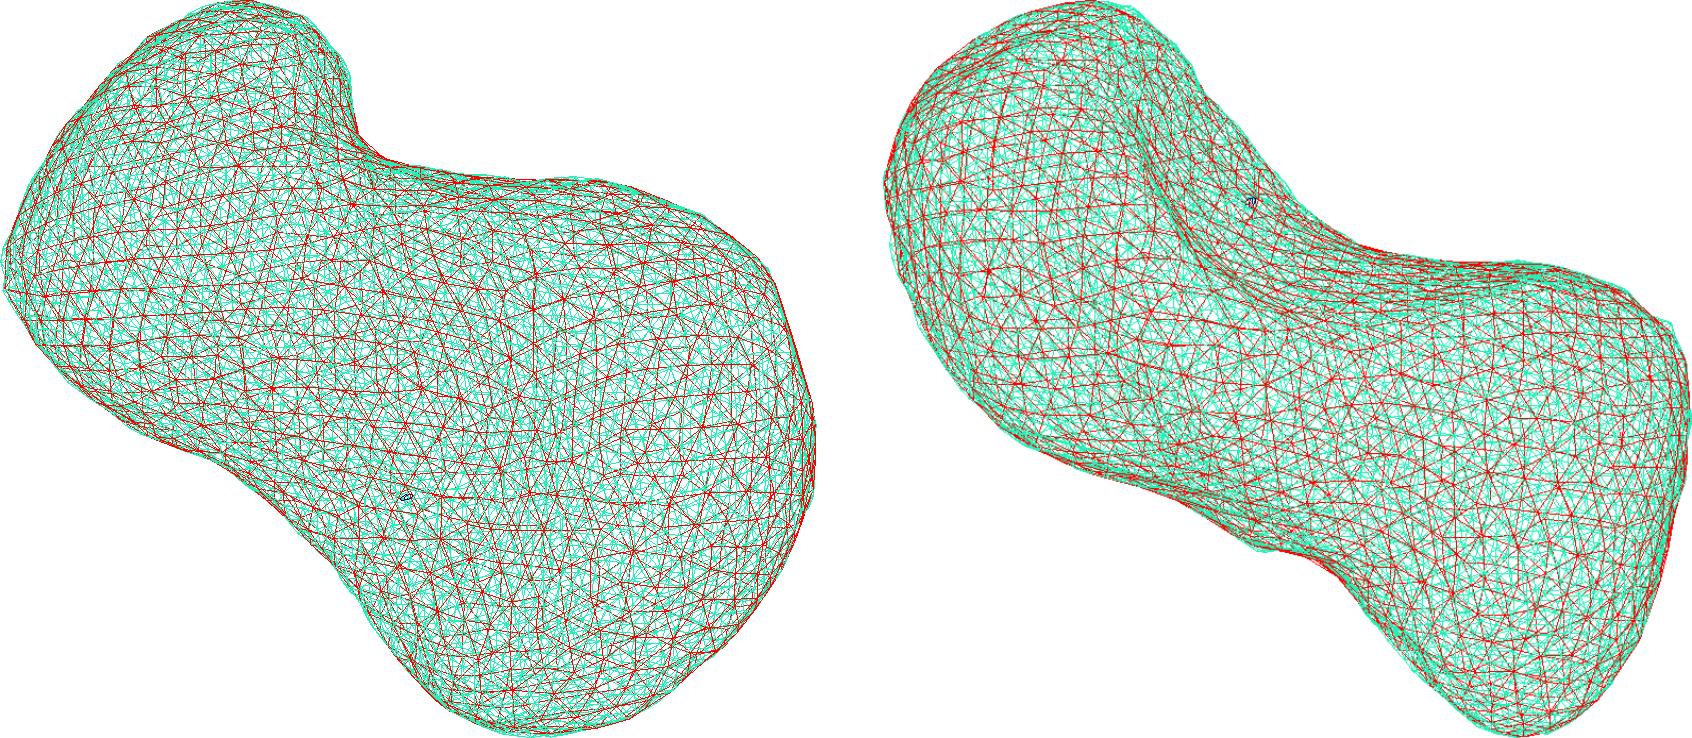
\includegraphics[width=0.9\textwidth]{\RootDir{img/wireframe_sca_color.png}}
		\caption{Scaphoid}
	\end{subfigure}
	~
	\begin{subfigure}[b]{\textwidth}
		\centering
		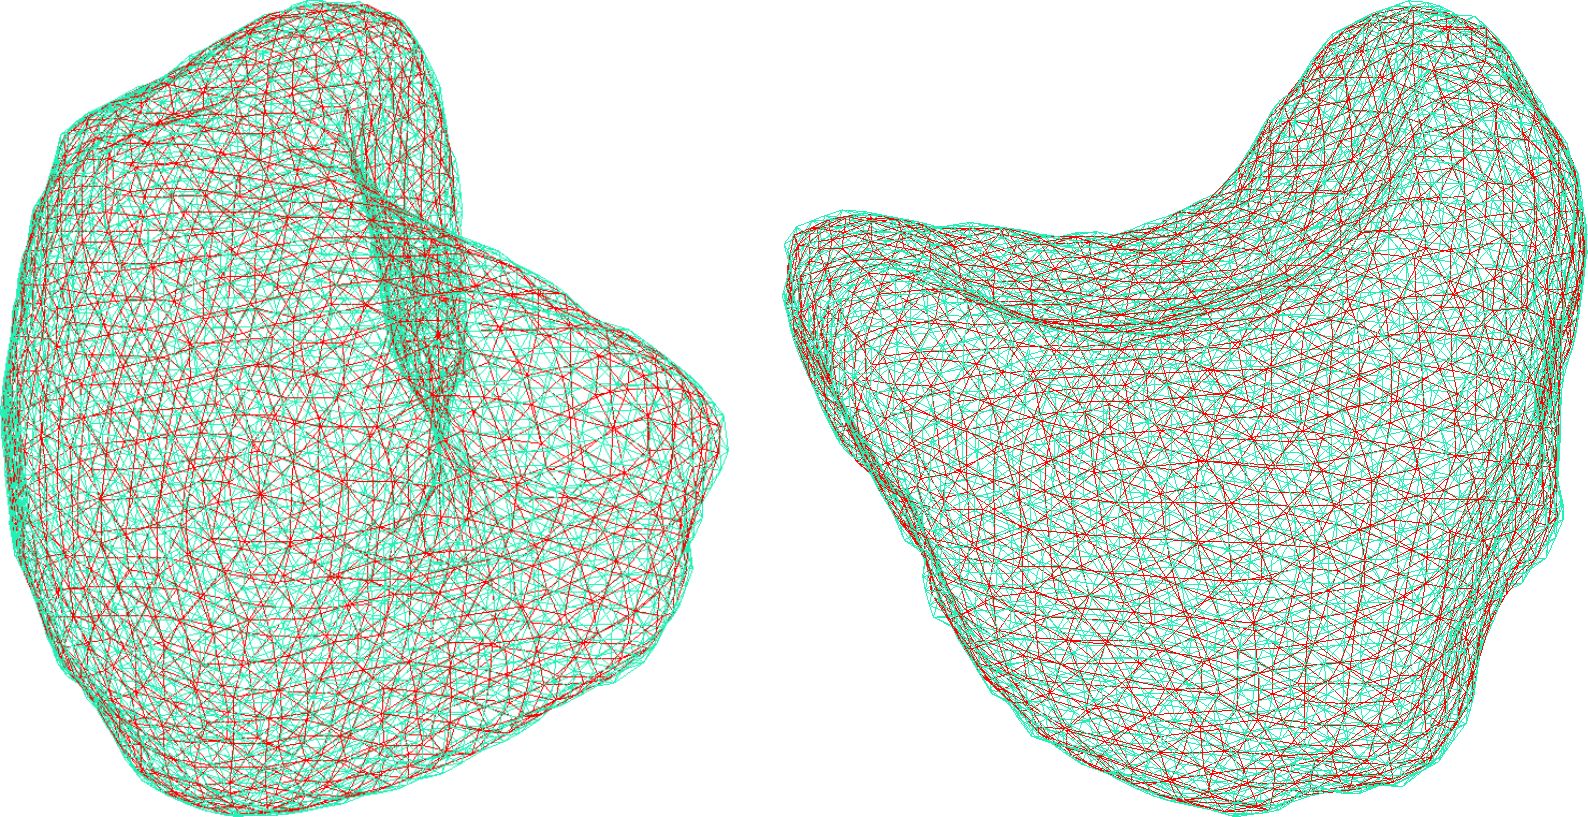
\includegraphics[width=0.8\textwidth]{\RootDir{img/wireframe_lun_color.png}}
		\caption{Lunate}
	\end{subfigure}
	
	\caption[Similarity between final and target meshes in wireframe view]{Two overlays of a database mesh \mr* in green and its registered template \mw* in red, in wireframe view. Both pairs were taken at two different angles. }
	\label{im:3_similar_wireframe}
\end{figure}


%% Fig: similarité en vue complète
\begin{figure}[!ht]
	\centering
	\begin{subfigure}[b]{\textwidth}
		\centering
		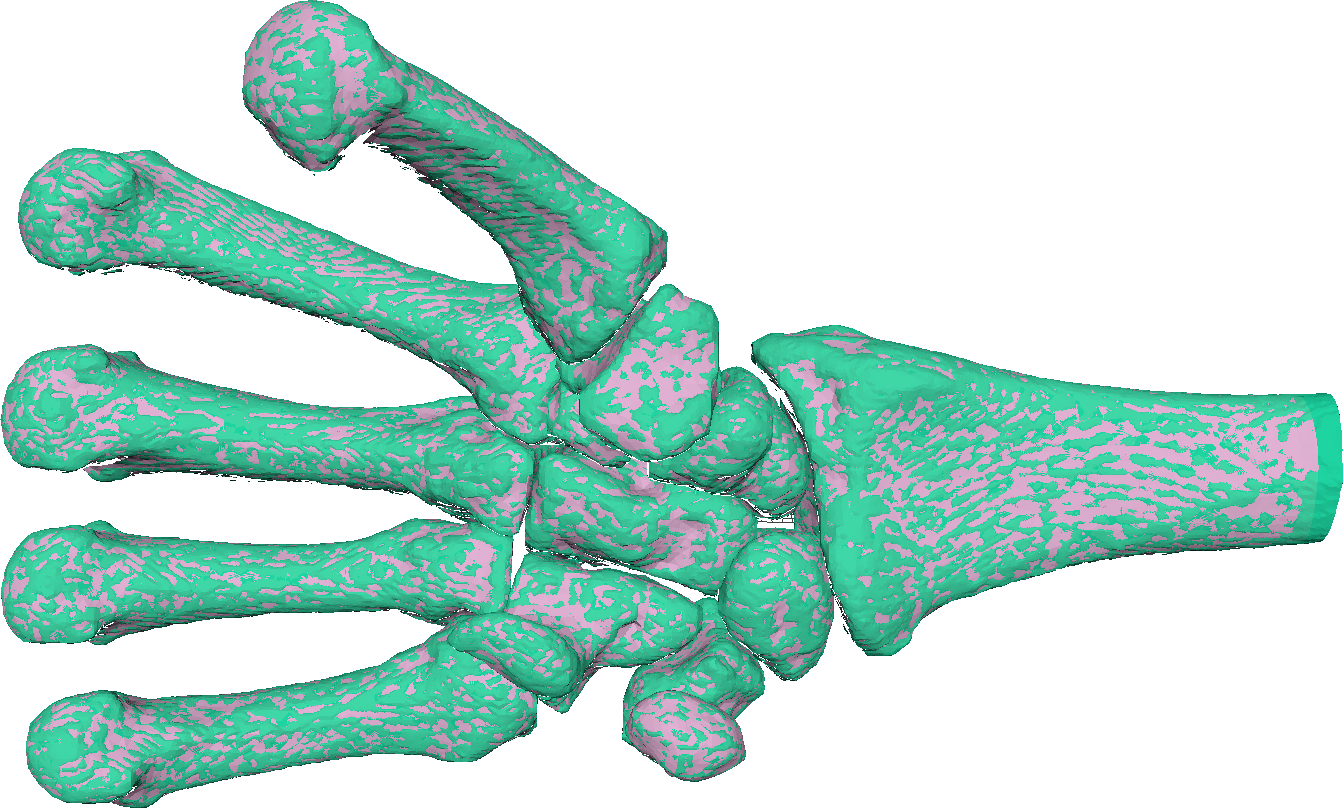
\includegraphics[width=0.9\textwidth]{\RootDir{img/deformed_1.png}}
		\caption{Person 1}
	\end{subfigure}
	~
	\begin{subfigure}[b]{\textwidth}
		\centering
		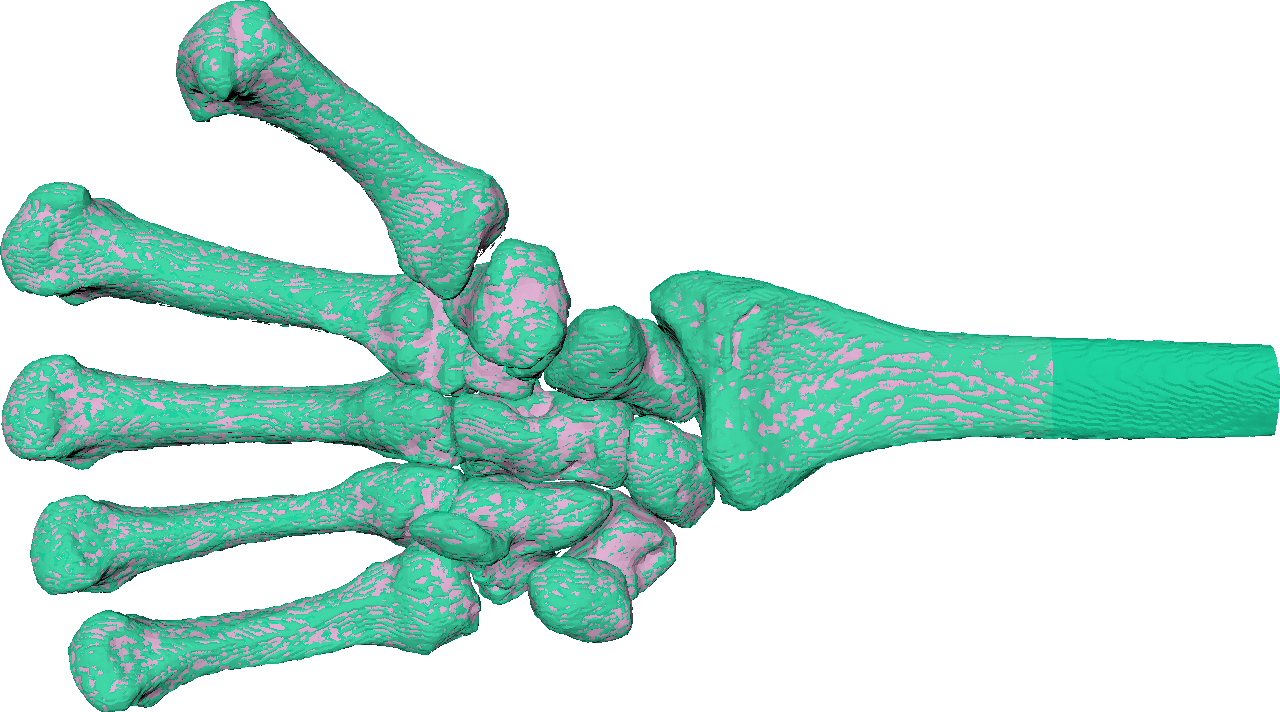
\includegraphics[width=\textwidth]{\RootDir{img/deformed_2.png}}
		\caption{Person 2}
	\end{subfigure}
	
	\caption[Similarity between final and target meshes as colored surfaces]{Two  database wrists and their registered meshes as colored surfaces. In green are the database target bones while the registered templates are colored pink.}
	\label{im:3_similar_colors}
\end{figure}
